\section{Simulations}
This work employs \Cyclus \cite{huff_fundamental_2016} to simulate the transition
from \glspl{LWR} to advanced nuclear reactors. This allows for deployment of 
reactors to meet any required energy 
demand, as well as material transactions between facilities. Each scenario
in this section models a once-through fuel cycle to a different subset of 
advanced reactor. Figure \ref{fig:fuel_cycle} shows the facilities 
and flow of materials in these scenarios. Facilities in red are used in scenarios 
with \gls{HALEU} fueled reactors, and provide a separation between the 
\gls{LEU} and \gls{HALEU} material streams. 

\begin{figure}
    \centering
    \begin{tikzpicture}[node distance=1.5cm]
        \node (mine) [facility] {Uranium Mine};
        \node (mill) [facility, below of=mine] {Uranium Mill};
        \node (conversion) [facility, below of=mill] {Conversion};
        \node (enrichment) [facility, below of=conversion]{Enrichment};
        \node (fabrication) [facility, below of=enrichment]{Fuel Fabrication};
        \node (reactor) [facility, below of=fabrication]{Reactor};
        \node (adv_reactor) [transition, right of=reactor, xshift=3cm]{Advanced Reactor};
        \node (wetstorage) [facility, below of=reactor]{Wet Storage};
        \node (drystorage) [facility, below of=wetstorage]{Dry Storage};
        \node (sinkhlw) [facility, below of=drystorage, xshift=5cm]{HLW Sink};
        \node (sinkllw) [facility, right of=enrichment, xshift=3cm]{LLW Sink};

        \draw [arrow] (mine) -- node[anchor=east]{Natural U} (mill); 
        \draw [arrow] (mill) -- node[anchor=east]{U$_3$O$_8$}(conversion); 
        \draw [arrow] (conversion) -- node[anchor=east]{UF$_6$}(enrichment);
        \draw [arrow] (enrichment) -- node[anchor=east]{Enriched U}(fabrication);
        \draw [arrow] (enrichment) -- node[anchor=south]{Tails}(sinkllw);
        \draw [arrow] (fabrication) -- node[anchor=east]{Fresh UOX}(reactor);
        \draw [arrow] (fabrication) -- node[anchor=west]{TRSIO fuel}(adv_reactor);
        \draw [arrow] (reactor) -- node[anchor=east]{Spent UOX}(wetstorage);
        \draw [arrow] (wetstorage) -- node[anchor=east]{Cool Spent UOX}(drystorage);
        \draw [arrow] (drystorage) -- node[anchor=east]{Casked Spent UOX}(sinkhlw);
        \draw [arrow] (adv_reactor) -- node[anchor=west]{Spent TRISO Fuel}(sinkhlw);

        \end{tikzpicture}
    \caption{Fuel cycle facilities and material flow between facilities. Facilities in 
    red are added in for the transition scenarios.}
    \label{fig:fuel_cycle}
\end{figure}

Multiple scenarios are considered in this work, with each scenario differing
by the type(s) of advanced reactor deployed and the power demand. The first 
scenario considered 
is the current fuel cycle in the U.S. starting in 1965. This fuel cycle 
consists of only \glspl{LWR}
and has no specified power demand. This scenario provides a baseline for 
the resource requirements that are currently used. Start and 
end dates for each \gls{LWR} were obtained from the \gls{IAEA} \gls{PRIS} database 
\cite{noauthor_power_1989}. Reactors still in operation in December 2020, and thus 
lacking an end date in the \gls{PRIS} database are assumed to operate through their 
current operating license 
\cite{noauthor_initial_2021,noauthor_second_2021,noauthor_watts_2021,noauthor_watts_2021-1,noauthor_clinton_2021,noauthor_comanche_2021,noauthor_comanche_2021-1,noauthor_perry_2021}. 
Only reactors with a power level above 400 MWe were used in the simulation 
to avoid including prototype and research reactors present in the database. 
Approximate masses for fuel used in the core the \gls{LWR}s was obtained 
from \cite{todreas_nuclear_2012} and \cite{cacuci_handbook_2010}. 

The other scenarios model a transition to at least one advanced reactor 
that requires \gls{HALEU}. Two different assumptions are applied about the growth 
in nuclear energy demand: one assuming no growth and the other assuming 
1\% annual growth. The transition to the new reactor type starts in 2025. 
These scenarios use the same  
non-reactor facilities as the simulation of the current 
U.S. fuel cycle. \gls{HALEU} fuel reactors 
considered include the \gls{USNC} \gls{MMR}
\cite{mitchell_usnc_2020} and the X-Energy Xe-100 
\cite{harlan_x-energy_2018}\cite{hussain_advances_2018}. Both of 
these reactors are designed 
to use \gls{HALEU} fuel in the form of \gls{TRISO} fuel particles. Table 
\ref{tab:reactor_summary} summarizes important design aspects of these two reactors.

\begin{table}[ht]
    \centering
    \caption{Mico-reactor design specifications}
    \label{tab:reactor_summary}
    \begin{tabular}{p{5cm}p{3cm}p{3cm}p{3cm}}
        \hline
        Design Criteria & \gls{USNC} \gls{MMR} & 
            X-energy Xe-100 & NuScale VOYGR \\\hline
        Reactor type & Modular HTGR & Modular HTGR & \\
        Power Output (MWth) & 15 & 200 & \\
        Enrichment (\% $^{235}U$) & 13 & 15.5 & \\
        Cycle Length (years) & 20 & online refuel &\\
        Fuel form & \gls{TRISO} compacts & \gls{TRISO} pebbles &\\
        Fuel burnup (MWd/MTU) & & & \\
        Reactor Lifetime & 20 years & 60 years & \\
        \hline
    \end{tabular}
\end{table}
    
The information available about these reactor designs in the public 
domain led to their selection for this work. Comparing the transitional \gls{HALEU} 
demands of these reactors will also inform the fuel cycle support 
implications of deploying reactors with long cycle 
times versus those utilizing online refueling. 

The transition scenarios investigated model the transition to multiple 
combinations of these reactors and different energy demand scenarios, 
summarized in Table \ref{tab:scenarios_once-through}

\begin{table}[ht]
    \centering
    \caption{Summary of the once-through fuel cycle transition scenarios.}
    \label{tab:scenarios_once-through}
    \begin{tabular}{l l l}
            \hline
            Scenario Number & Reactors Present & Energy growth model\\\hline
            1 & \glspl{LWR} & N/A \\
            2 & \glspl{LWR} and \gls{USNC} \gls{MMR} & No growth \\
            3 & \glspl{LWR} and X-energy Xe-100& No growth \\
            4 & \glspl{LWR}, X-energy Xe-100, \gls{USNC} \gls{MMR}& No growth\\
            5 & \glspl{LWR}, \gls{USNC} \gls{MMR}, NuScale VOYGR & No growth\\
            6 & \glspl{LWR}, X-energy Xe-100, NuScale VOYGR & No growth\\
            7 & \glspl{LWR}, X-energy Xe-100, \gls{USNC} \gls{MMR}, NuScale VOYGR & No growth\\
            8 & \glspl{LWR} and \gls{USNC} \gls{MMR}& 1\% growth \\
            9 & \glspl{LWR} and X-energy Xe-100& 1\% growth\\
            10 & \glspl{LWR}, X-energy Xe-100, \gls{USNC} \gls{MMR}& 1\% growth\\
            11 & \glspl{LWR}, \gls{USNC} \gls{MMR}, NuScale VOYGR & 1\% growth\\
            12 & \glspl{LWR}, X-energy Xe-100, NuScale VOYGR & 1\% growth\\
            13 & \glspl{LWR}, X-energy Xe-100, \gls{USNC} \gls{MMR}, NuScale VOYGR & 1\% growth\\

    \end{tabular}
\end{table}

The \glspl{LWR} in all of the simulations are deployed 
at their respective time steps using a ``cycamore:DeployManagerInst'' institution, 
and the advanced recators are deployed as needed by a ``cycamore:DeployInst''
institution \cite{scopatz_cyclus_2015}. Both of these institutions are within the same 
``cycamore:GrowthRegion'' region, which specifies the energy demand for the simulation.

Material compositions are defined using recipes. Recipes for materials in the fuel 
cycle prior to the reactors (e.g. natural uranium, enriched urnaium) are defined 
soley by the uranium isotope ratios. Recipes for the fresh and 
spent fuel for the \glspl{LWR} was found in \cite{yacout_visionverifiable_2006}.
The spent \gls{LWR} fuel recipe defines the composition of the cool spent UOX and 
the casked spent UOX. The recipe for \gls{TRISO} fuel is defined by the uranium 
isotopic ratio. The spent \gls{TRISO} fuel is defined based on depletion models of 
the reactor cores.  


Each of the once-through transition scenarios are compared on multiple 
criteria: the number of advanced reactors deployed, the energy profile, 
the mass of enriched 
uranium required, the amount of \gls{SWU} capacity required to enrich uranium,
and the mass of waste produced. 

\subsection{Scenario 1}
Scenario 1 models only the \glspl{LWR} deploying the United States with no 
perscribed energy demand. As expected, the energy 
produced by the \glspl{LWR} follows with the number of reactors deployed
(Figure \ref{fig:energy1}). The maximum number of \glspl{LWR} deployed is 
, and reactors are deployed in 2025. 

I can compare some of these results to EIA data on power produced and 
uranium purchases from domestic suppliers \cite{us_eia_monthly_2022}.

\begin{figure}
    \centering
    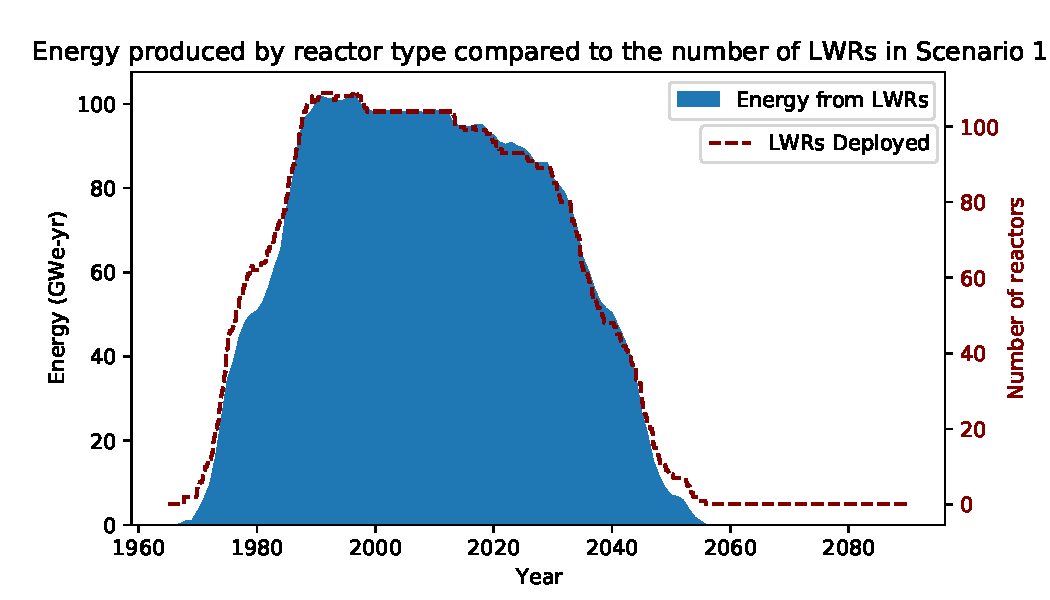
\includegraphics{energy_scenario1.pdf}
    \caption{Energy produced and the number of reactors deployed in Scenario 1.}
    \label{fig:energy1}
\end{figure}

\subsection{Reactor deployment}

\subsection{Uranium resources}

\subsection{SWU capacity}

\subsection{Waste}